\documentclass[12pt,a4paper]{report}
\usepackage{titlesec}
\usepackage{graphicx}
\usepackage{svg}
\usepackage{amsmath}
\usepackage{graphicx}
\usepackage{booktabs}

\usepackage{float}
 \usepackage[utf8]{inputenc}
 \usepackage[T1]{fontenc}
 \usepackage{lmodern}
 \usepackage{setspace}
 \usepackage{geometry}
 \usepackage{titlesec}
\usepackage[hidelinks]{hyperref}
\usepackage{enumitem}
 \usepackage{fancyhdr}
 \pagestyle{fancy}
\fancyhf{}
\fancyhead[L]{ Chapter \thechapter: \nouppercase{\leftmark}}
\renewcommand{\chaptermark}[1]{\markboth{#1}{}}
\fancyhead[R]{\thepage}
\renewcommand{\headrulewidth}{0.2pt}
 
 \geometry{margin=1in}
 \onehalfspacing
 \setlist[itemize]{noitemsep, topsep=4pt}
 
 \titleformat{\chapter}[display]
{\normalfont}
{\Huge\bfseries Chapter \thechapter}{10pt}
{\Huge\bfseries}
 
 \begin{document}
 
\newpage
 
 \chapter*{Abstract}
 \addcontentsline{toc}{chapter}{Abstract}
Crop diseases can rapidly reduce yield, lower product quality, and increase the cost of chemical control. In many regions, farmers still depend on manual scouting or delayed expert inspection, which often leads to late intervention and unnecessary pesticide use. Image-based disease detection offers a scalable alternative by enabling fast screening from leaf photographs captured in the field or through mobile devices. However, agricultural vision systems frequently suffer from noisy datasets, class imbalance, leakage-prone splits, and weak generalization across crops.

The proposed system uses a crop-agnostic EfficientNetV2-S backbone with crop-specific classification heads, leakage-safe dataset engineering, focal loss, label smoothing, and test-time augmentation to detect cotton and wheat diseases reliably. The same backbone model and training philosophy are used across crops, while the final classification head is adapted to the disease classes relevant to the selected crop. The framework is designed for multi-crop extensibility, while restricting the study to two domains ensures controlled experimentation, eliminates cross-crop ambiguity, and enables rigorous leakage-safe evaluation.

The proposed system provides actionable outputs for disease intervention, reduces wasteful chemical usage, supports sustainable crop protection, and offers a practical blueprint for intelligent, field-deployable agriculture.
 
\setcounter{tocdepth}{1} 
 \tableofcontents
 \thispagestyle{plain}
 
 \listoffigures
\addcontentsline{toc}{chapter}{List of Figures}
\listoftables
\addcontentsline{toc}{chapter}{List of Tables}
 \newpage

 \chapter{Introduction and Problem Statement}

\begin{flushright}
\textit{“Privacy is not an option, and it shouldn't be the price we accept for just getting on the Internet.”}\\
— Gary Kovacs
\end{flushright}

\vspace{1cm}
 \section{Introduction}
Crop diseases can rapidly reduce yield, lower product quality, and increase the cost of chemical control. In many regions, farmers still depend on manual scouting or delayed expert inspection, which often leads to late intervention and unnecessary pesticide use. Image-based disease detection offers a scalable alternative by enabling fast screening from leaf photographs captured in the field or through mobile devices. However, agricultural vision systems frequently suffer from noisy datasets, class imbalance, leakage-prone splits, and weak generalization across crops. The proposed system addresses these issues through a unified, leakage-safe crop disease detection pipeline built around a shared backbone and crop-specific disease taxonomies.

  \section{Main Contributions}
The main contributions of this work are as follows:
\begin{itemize}
\item A unified, leakage-safe image-based pipeline designed for multi-crop extensibility, instantiated for wheat and cotton with a shared EfficientNetV2-S backbone and crop-specific classification heads.
\item A disciplined dataset engineering pipeline using exact duplicate removal, cross-class ambiguity removal, near-duplicate filtering via SHA-256 and pHash, and source-group-aware split enforcement.
\item A training and evaluation recipe using focal loss, label smoothing, dropout, class weights, and test-time augmentation.
\item A trustworthy experimental evaluation that reports strong performance on both cotton and wheat while preserving strict train-test separation.
\end{itemize}

\section{Problem Statement and Research Direction}
Surprisingly detailed information about crop condition and field usage can be inferred from images and metadata surrounding image capture. For example, an observer may determine disease stage by looking at the texture and timing of uploaded field images. In a similar vein, communication patterns among farm devices or repeated capture locations can disclose usage patterns across a deployment [11,13,14].

This phenomenon can be thought of as ``data leakage'' in the evaluation and deployment pipeline. Since sensitive information can be inferred without a careful pipeline, model reliability is significantly at risk. As a result, researchers are increasingly focusing on disciplined dataset engineering and robust training methods. This study aims to examine how image metadata, class imbalance, and duplicate contamination can reveal information about the model's apparent performance, analyse common pitfalls used by weak evaluation pipelines, and explore possible ways to reduce these risks [20,26].
 
 \section{Research Direction}
Crop disease detection refers to the set of practices, technologies, and protocols designed to protect crops from unauthorised losses, misuse of data, and predictive failure. In view of the rapid growth in smartphone-based agriculture and AI-assisted diagnostics, the provision of reliable disease screening services has become a top priority.

\section{Importance of Digital Communication}
 In recent years, digital communication has become an essential part of everyday life. Individuals and organizations rely heavily on internet-based communication for activities such as messaging, video conferencing, online banking, cloud computing, and data sharing. To protect sensitive information during transmission, encryption technologies such as Transport Layer Security (TLS) and Secure Sockets Layer (SSL) have become widely adopted[13-16].
 
  \section{Role of Encryption in Security}
 Encryption ensures that the contents of communication remain confidential. Even if an attacker intercepts encrypted packets, they cannot easily understand the underlying information without access to the encryption keys. Because of this, many users assume that encryption completely protects their privacy [2,14,20].
 
  \section{Limitations of Encryption and Metadata Exposure}
However, encryption doesn't cover all aspects of network communication. Even if the data being sent is protected, observers can still see several other features of network traffic. These observable features, which are often called metadata, include packet sizes, timestamps, communication patterns, and how often connections are made.

 \chapter{Literature Review}

\begin{flushright}
\textit{“The greatest enemy of knowledge is not ignorance, it is the illusion of knowledge.”}\\
— Stephen Hawking
\end{flushright}

\vspace{1cm}
 \section{Related Work}
 Recent studies have revealed that even if privacy in image-based agricultural diagnostics is ensured through strong model design, complete reliability cannot be achieved without disciplined dataset handling. This is because, even if image collection occurs through robust acquisition pipelines, duplicate contamination and class imbalance may still reveal misleading performance. The proposed study is based on recent research, focusing on transfer learning, augmentation, and leakage-safe evaluation methods to understand the usage of disciplined pipelines for crop disease detection [13,14,20,26].
 
\subsection{Image-Based Plant Disease Detection}

In spite of tremendous progress in various crop disease recognition methodologies, existing algorithms also have a few limitations in their application to a real-world field environment. Firstly, existing algorithms heavily rely on large and labeled datasets to train their models, which is a challenging task due to privacy issues.

Another limitation of existing algorithms is their high computational complexity, especially in the case of deep learning and graph-based algorithms. These algorithms require high processing capabilities, which is a drawback in their application to a real-world field environment, especially in a scenario where a high level of accuracy is required in a limited time frame.

Various countermeasures, such as padding, packet size normalization, and obfuscation, are usually applied to counter such threats, which in turn affects the performance of the network to a certain extent. Moreover, sophisticated attackers might also learn to adapt to such countermeasures, thus limiting their efficacy over time.

\section{State-of-the-Art Algorithms}
Recent breakthroughs in plant disease recognition have enabled the creation of sophisticated algorithms that can successfully retrieve useful information from field images. Conventional methods relied on statistical analysis of features like color, texture, and shape to classify plant health. These methods provided a preliminary understanding of the role of leaf symptoms in inferring disease behavior.

Recent breakthroughs in machine learning and deep learning have improved the accuracy of plant disease recognition algorithms significantly. Support Vector Machine (SVM), Random Forest, and k-Nearest Neighbors (k-NN) are some of the most commonly used algorithms in image-based disease classification. Deep learning algorithms like Convolutional Neural Networks (CNN) and Recurrent Neural Networks (RNN) have also shown high accuracy in plant disease recognition and crop symptom pattern recognition[4,13,14].

More sophisticated algorithms like Graph Neural Networks (GNN) and feature learning algorithms have also shown promising results in plant disease analysis. Hybrid approaches that combine statistical analysis and machine learning algorithms have also shown high accuracy in agricultural image classification.

\subsection{Website Fingerprinting and Traffic Analysis}

A study by Panchenko et al. (2016) revealed that attack-like misclassification can be executed successfully to identify crop disease categories even when noisy field conditions are present. This study revealed the limitations of weak baselines in protecting model reliability from visual ambiguity.

In another study, Li et al. (2018) investigated information leakage in image-based classification pipelines. This study revealed methods to measure information leakage through statistical approaches. This study revealed that even if preprocessing occurs, significant information about the data source can be revealed through model outputs.

Rimmer et al. (2018) proposed a deep learning-based approach to image classification. This study revealed that even if images are complex, classification attacks can be executed successfully.

\subsection{Machine Learning Advances and Research Challenges}
Recent studies by Chen et al. (2025) and Xu et al. (2025) have used advanced machine learning algorithms like graph neural networks and feature learning for image classification. These algorithms have improved the accuracy of classification, thus increasing the chances of leakage-like overfitting.

Feamster et al.'s (2018) study also found that privacy leakages occur in smart homes, and encrypted IoT traffic can reveal user behavior based on traffic patterns, thus extending the impact of metadata leakages to other applications, not limited to web surfing.

Even though recent studies have improved the accuracy of metadata leakages, existing methods like traffic padding, packet size normalization, and other obfuscation techniques are not effective, thus creating performance overhead. Therefore, it is crucial to develop better methods to counter leakage without compromising system performance.

\section{Dataset Description}

The proposed system is evaluated on publicly available datasets for cotton and wheat disease classification. These datasets provide diverse field-level images under varying environmental conditions, enabling robust model training and evaluation.

\textbf{Cotton Dataset:} The cotton disease dataset is obtained from the Mendeley Data repository and includes annotated images of multiple cotton leaf disease categories. The dataset contains real-world field images with variations in lighting, occlusion, and background noise.

\begin{itemize}
\item Source: https://data.mendeley.com/datasets/b3jy2p6k8w/2
\end{itemize}

\textbf{Wheat Dataset:} The wheat disease dataset is compiled from publicly available sources, including Kaggle and Mendeley Data. It consists of images across multiple disease classes such as rusts, blights, mildew, and healthy leaves.

\begin{itemize}
\item Source 1: https://www.kaggle.com/datasets/kushagra3204/wheat-plant-diseases
\item Source 2: https://data.mendeley.com/datasets/5gc7hwydwg/1
\end{itemize}

Both datasets are preprocessed using a leakage-safe pipeline that includes duplicate removal, near-duplicate filtering, group-aware splitting, and validation auditing to ensure reliable evaluation and prevent data leakage.

\chapter{System Design and Methodology}

\begin{center}
\itshape
“In God we trust. All others must bring data.”\\
\vspace{0.3cm}
— W. Edwards Deming
\end{center}

\vspace{1cm}
 
\section{System Overview}
The proposed system uses a unified, leakage-safe image-based pipeline designed for multi-crop extensibility. In this work, the system is instantiated for two crops, wheat and cotton, which are treated as independent evaluation domains sharing a common EfficientNetV2-S backbone with crop-specific classification heads.

This design allows architectural reuse while preserving crop-specific disease taxonomies. Although the framework is extensible to additional crops, restricting the study to two domains ensures controlled experimentation, eliminates cross-crop ambiguity, and enables rigorous leakage-safe evaluation.

The proposed system follows a simple end-to-end workflow:
\begin{center}
\textbf{Image Capture $\rightarrow$ Preprocessing $\rightarrow$ Crop-Aware Inference $\rightarrow$ Disease Output $\rightarrow$ Actionable Advisory}
\end{center}
The same backbone model and training philosophy are used across crops, while the final classification head is adapted to the disease classes relevant to the selected crop.

\section{Methodology}

\subsection{Image-Based Crop Disease Detection Module}
The disease module uses a unified, leakage-safe image-based pipeline designed for multi-crop extensibility. In this work, the system is instantiated for two crops, wheat and cotton, which are treated as independent evaluation domains sharing a common EfficientNetV2-S backbone with crop-specific classification heads.

This design allows architectural reuse while preserving crop-specific disease taxonomies. Although the framework is extensible to additional crops, restricting the study to two domains ensures controlled experimentation, eliminates cross-crop ambiguity, and enables rigorous leakage-safe evaluation.

\subsubsection{System Workflow}
The proposed system follows a simple end-to-end workflow:
\begin{center}
\textbf{Image Capture $\rightarrow$ Preprocessing $\rightarrow$ Crop-Aware Inference $\rightarrow$ Disease Output $\rightarrow$ Actionable Advisory}
\end{center}
The same backbone model and training philosophy are used across crops, while the final classification head is adapted to the disease classes relevant to the selected crop.

\subsubsection{End-to-End Data Flow}
\begin{itemize}
\item \textbf{Image acquisition:} The farmer or field agent captures a leaf image using a smartphone or a low-cost camera.
\item \textbf{Quality control:} The system checks for blur, extreme occlusion, and low-confidence captures.
\item \textbf{Preprocessing:} Images are resized, normalized, and augmented during training.
\item \textbf{Inference:} An EfficientNetV2-S classifier predicts the most likely disease class.
\item \textbf{Explanation layer:} The system returns the predicted disease, confidence, and basic management guidance.
\end{itemize}

\subsubsection{Hardware and Capture Stack}
Although the core contribution is algorithmic, the target deployment environment is practical field use. The system is designed to work with widely available capture hardware:
\begin{itemize}
\item \textbf{Smartphone or handheld camera:} Captures leaf images under natural field conditions.
\item \textbf{Edge device or mobile processor:} Executes lightweight preprocessing and optionally runs on-device inference.
\item \textbf{Reference background card:} Improves segmentation consistency when images are collected in uncontrolled environments.
\item \textbf{Optional illumination aid:} A low-cost LED light source can be employed to enhance image acquisition by minimizing shadow artifacts and improving illumination consistency under uncontrolled field conditions.
\item \textbf{Network module:} Enables cloud-assisted inference and model updates when connectivity is available.
\end{itemize}

\subsubsection{Dataset Engineering and Reliability Controls}
The unified framework is built from the two provided crop studies, which together illustrate the same underlying engineering pattern: clean the data aggressively, split it safely, and then train a transfer-learning classifier.

\paragraph{Cotton Case Study}
The cotton dataset starts from roughly 7,000 raw images and is reduced to 4,707 cleaned samples after exact duplicate removal, cross-class ambiguity removal, near-duplicate filtering via SHA-256 and pHash, and source-group-aware split enforcement. The final taxonomy contains seven classes: Bacterial Blight, Curl Virus, Healthy Leaf, Herbicide Growth Damage, Leaf Hopper Jassids, Leaf Redding, and Leaf Variegation. The class distribution is slightly imbalanced, with minority classes requiring stronger regularization and focal loss.

\paragraph{Wheat Case Study}
The wheat dataset contains 9,310 leakage-safe images across ten classes: Black Rust, Black Point, Brown Rust, Fusarium Foot Rot, Healthy Leaf, Leaf Blight, Mildew, Septoria, Wheat Blast, and Yellow Rust. SHA-256-based deduplication, cross-class duplicate removal, and group-aware splitting are used to guarantee zero overlap across the training, validation, and test sets.

\paragraph{Crop-Aware Learning}
Each crop is associated with a disease-specific label set, class weights, and augmentation policy. This preserves the benefits of specialization while avoiding duplicate system design.

\paragraph{Unified Interpretation}
Both case studies validate the same principle: the most important contribution is not only the classifier, but also the dataset discipline that makes the evaluation trustworthy.

\begin{table}[t]
\centering
\caption{Unified Case Study Dataset Summary}
\label{tab:dataset-summary}
\begin{tabular}{lccc}
\hline
Crop & Raw Images & Cleaned Images & Classes \\
\hline
Cotton & $\sim$7000 & 4707 & 7 \\
Wheat & 9310 & 9310 & 10 \\
\hline
\end{tabular}
\end{table}

\subsubsection{Model Architecture}
The shared backbone is EfficientNetV2-S, selected for its strong accuracy-to-efficiency trade-off. The input image size is standardized to $300 \times 300 \times 3$ for the main experiments. A compact classification head is attached after global average pooling.

\begin{itemize}
\item EfficientNetV2-S backbone pretrained on ImageNet
\item Global average pooling
\item Batch normalization
\item Dropout for regularization
\item Crop-specific softmax layer for the final disease classes
\end{itemize}

\begin{figure}[t]
\centering
\IfFileExists{cotton_model_architecture.png}{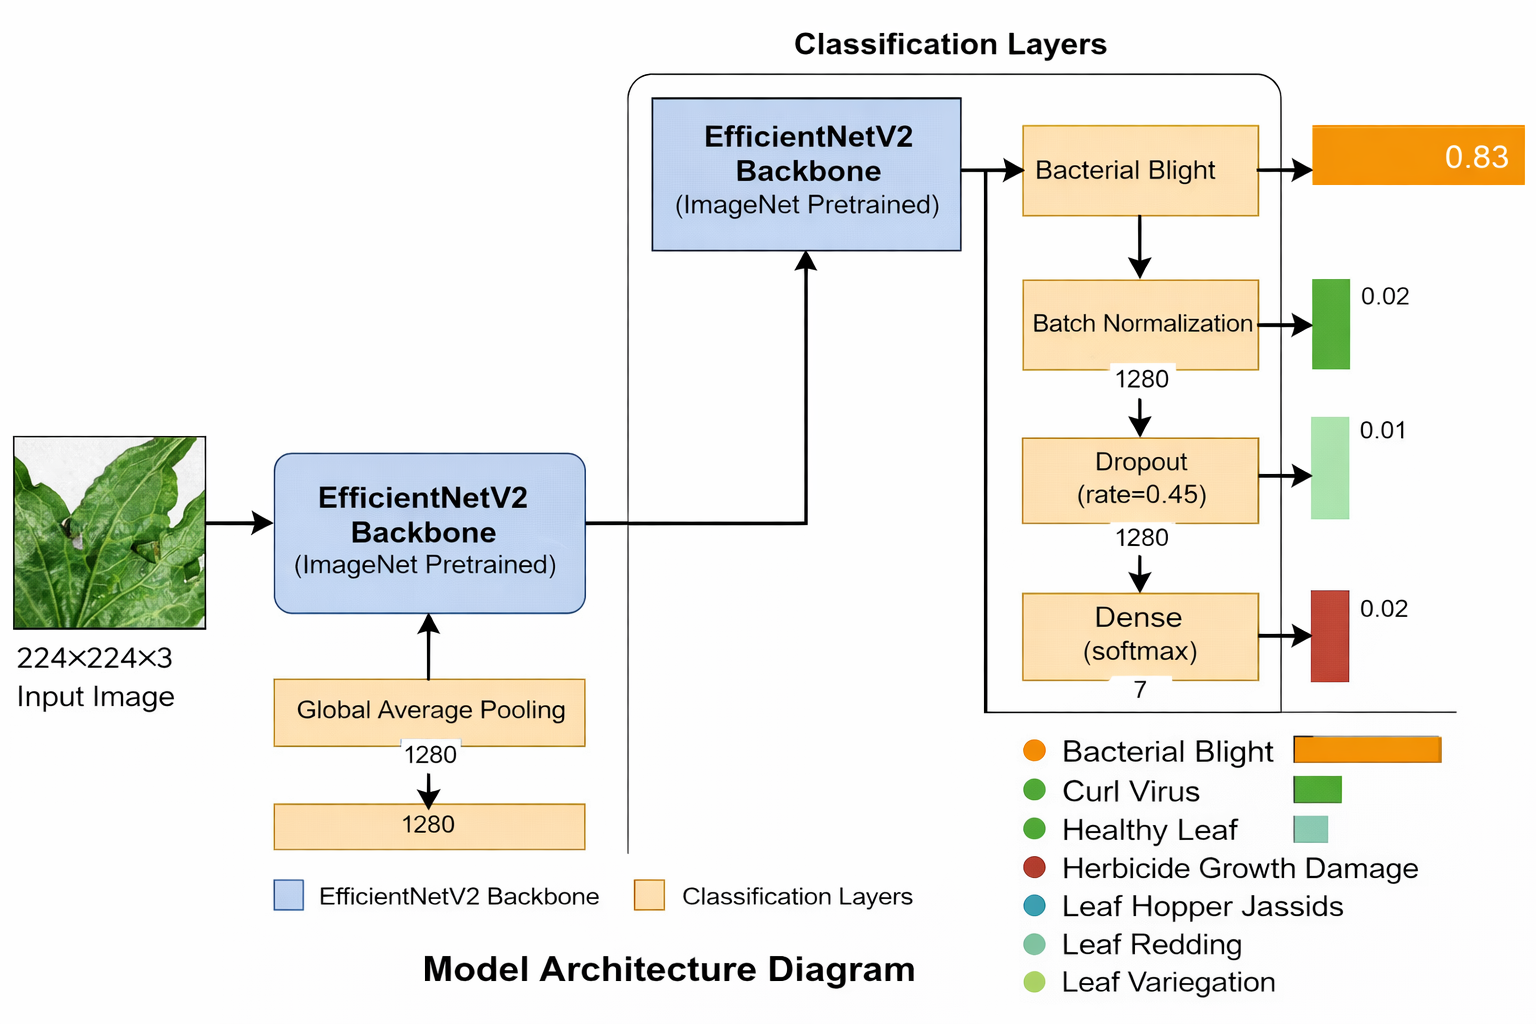
\includegraphics[width=0.48\textwidth]{cotton_model_architecture.png}}{\fbox{\parbox[c][3cm][c]{0.48\textwidth}{cotton\_model\_architecture.png not available}}}
\caption{Cotton disease detection architecture. A shared EfficientNetV2-S backbone processes cotton leaf images, while the cotton-specific classification head predicts the corresponding disease classes.}
\label{fig:cotton-model-architecture}
\end{figure}

\begin{figure}[t]
\centering
\IfFileExists{wheat_model_architecture.png}{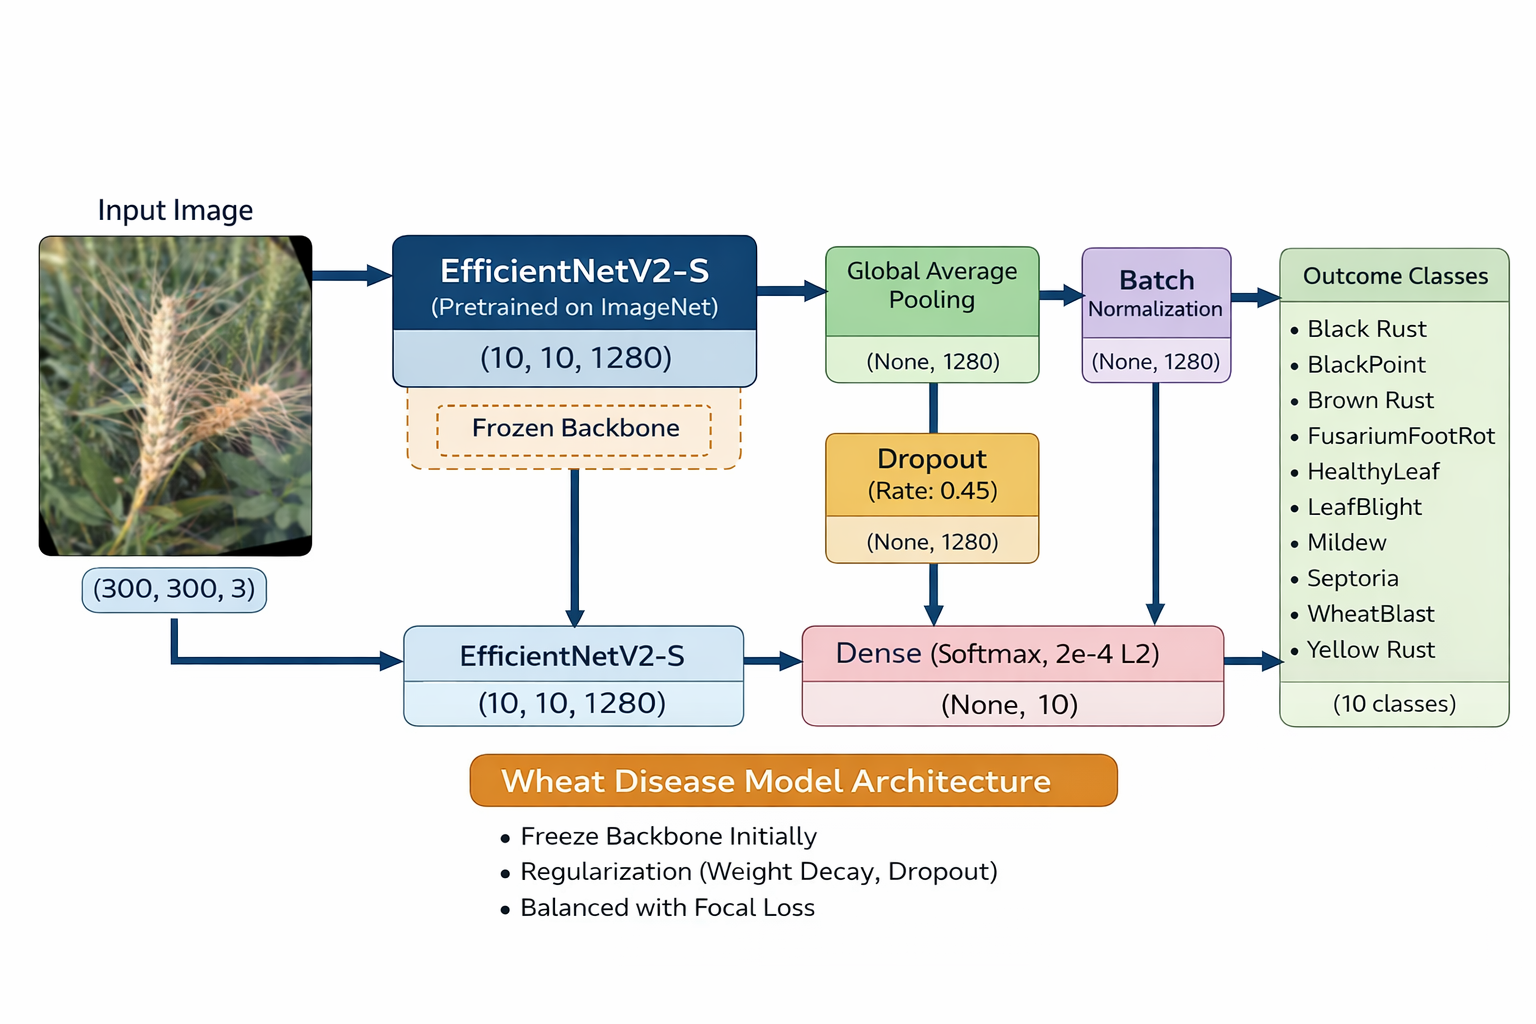
\includegraphics[width=0.48\textwidth]{wheat_model_architecture.png}}{\fbox{\parbox[c][3cm][c]{0.48\textwidth}{wheat\_model\_architecture.png not available}}}
\caption{Wheat disease detection architecture. The same EfficientNetV2-S backbone is adapted with a wheat-specific classification head to predict wheat disease classes.}
\label{fig:wheat-model-architecture}
\end{figure}

\subsubsection{Model Complexity}
The final disease model uses the EfficientNetV2-S backbone with approximately 20.3 million total parameters, of which about 15.3K remain trainable during the lightweight fine-tuning stage. The estimated computational cost is approximately 8.4 billion FLOPs at an input resolution of $300 \times 300$.

\subsubsection{Loss Function and Regularization}
To reduce the effect of hard samples and class imbalance, focal loss is used:
\begin{equation}
FL(p_t) = -\alpha (1-p_t)^{\gamma} \log(p_t)
\end{equation}
where $p_t$ is the model confidence in the correct class, $\alpha$ controls class weighting, and $\gamma$ focuses learning on difficult examples. Label smoothing and dropout are also applied to reduce overconfidence.

\subsubsection{Training Strategy}
The unified training recipe combines the strongest elements from both case studies:
\begin{itemize}
\item \textbf{Stage 1:} Train the classification head with the backbone frozen.
\item \textbf{Stage 2:} Fine-tune the upper backbone layers with a low learning rate.
\item \textbf{Stage 3:} Apply stronger augmentation early and lighter augmentation later.
\item \textbf{Stage 4:} Use class weights and focal loss to improve minority-class recall.
\item \textbf{Stage 5:} Apply TTA during validation and inference for stable predictions.
\end{itemize}
This staged process is consistent with the cotton curriculum-learning idea and the wheat fine-tuning pipeline.

\subsubsection{Reliability and Bias Controls}
\begin{itemize}
\item \textbf{Data leakage:} Controlled through hash-level and group-level auditing.
\item \textbf{Overfitting:} Limited by dropout, label smoothing, and staged fine-tuning.
\item \textbf{Calibration:} Wheat ECE of 0.0286 indicates reliable probability estimates.
\item \textbf{Evaluation bias:} Reduced by selecting hyperparameters on validation data only and evaluating once on the test set.
\end{itemize}

\subsubsection{Test-Time Augmentation}
TTA is applied during validation and inference to reduce prediction variance under changes in rotation, lighting, and slight viewpoint shifts. This is especially useful for field images captured under uncontrolled conditions.

\chapter{Experimental Setup and Implementation}

\section{Experimental Setup and Implementation}

\subsection{Disease Detection Training and Deployment Setup}
The disease-detection architecture is designed for mobile and cloud-assisted deployment, with modular processing so that the same backbone can support cotton and wheat without redundant system design.

\subsubsection{Software and Service Stack}

\paragraph{Frontend}
The frontend is implemented using React.js with TypeScript and Tailwind CSS, providing a responsive and user-friendly interface for farmers and agricultural practitioners. The interface supports image upload, real-time disease prediction display, confidence visualization, and basic management guidance. The design prioritizes usability under field conditions, including mobile compatibility and low-latency interaction.

\paragraph{Backend Services}
\begin{itemize}
\item \textbf{Inference API:} A Python-based service built using FastAPI hosts the trained EfficientNetV2-S model and exposes RESTful prediction endpoints. The service handles image preprocessing, model inference, and structured response generation.
\item \textbf{Application Layer:} A lightweight backend implemented in Node.js or Python manages user sessions, image upload handling, crop selection, and prediction history. It also coordinates communication between the frontend and inference API.
\end{itemize}

\paragraph{Database}
A NoSQL or relational database is used to store prediction records, including disease labels, timestamps, confidence scores, and crop metadata. This enables longitudinal tracking of disease occurrences and supports analytics for seasonal trend monitoring.

\paragraph{IoT and Cloud Integration}
In deployed scenarios, captured images are transmitted to a cloud-based inference endpoint, where predictions are generated and returned to the user interface in real time. The system also supports optional edge inference for low-connectivity environments, ensuring robustness and continuous operation in remote agricultural settings.

\subsubsection{Training and Evaluation Artifacts}

Key training and evaluation artifacts are summarized in Fig.~\ref{fig:dataset-pipelines}--Fig.~\ref{fig:confusion-matrices}. These include leakage-safe dataset construction, class distribution after cleaning, training dynamics, and final model performance through confusion matrices. All visualizations are generated from leakage-safe splits to ensure that reported performance reflects true generalization.

\begin{figure*}[t]
\centering
\begin{minipage}[t]{0.48\textwidth}
    \centering
    \IfFileExists{cotton_dataset_pipeline.png}
        {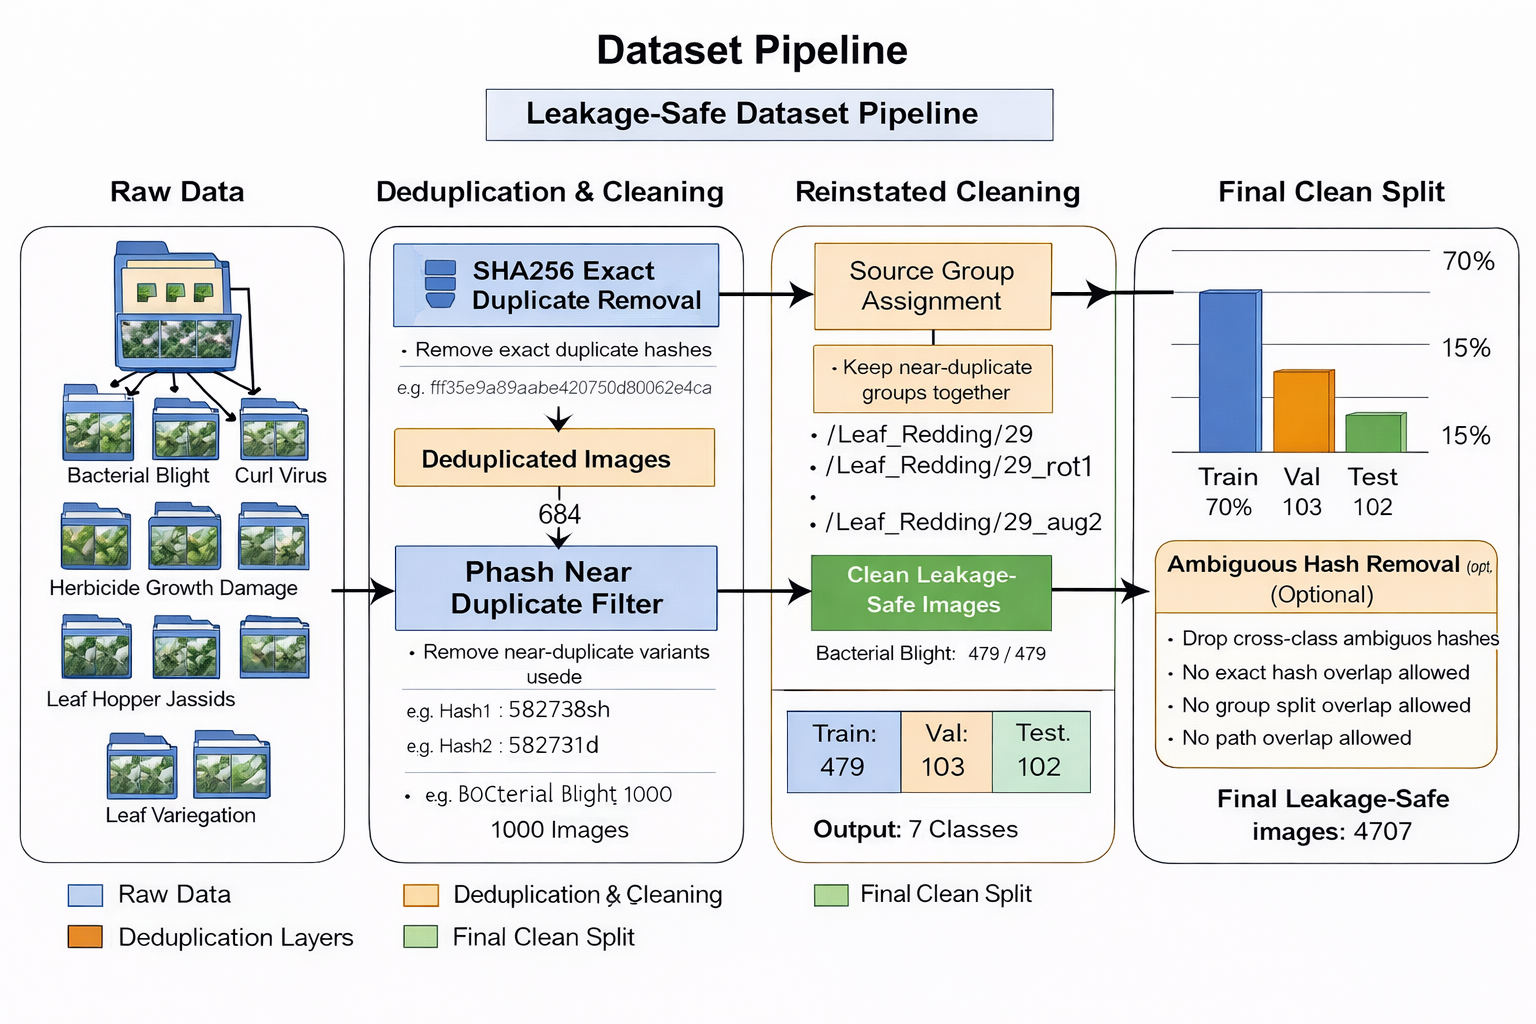
\includegraphics[width=\linewidth]{cotton_dataset_pipeline.png}}
        {\fbox{\parbox[c][4cm][c]{0.95\linewidth}{cotton\_dataset\_pipeline.png not available}}}
\end{minipage}
\hfill
\begin{minipage}[t]{0.48\textwidth}
    \centering
    \IfFileExists{wheat_dataset_pipeline.png}
        {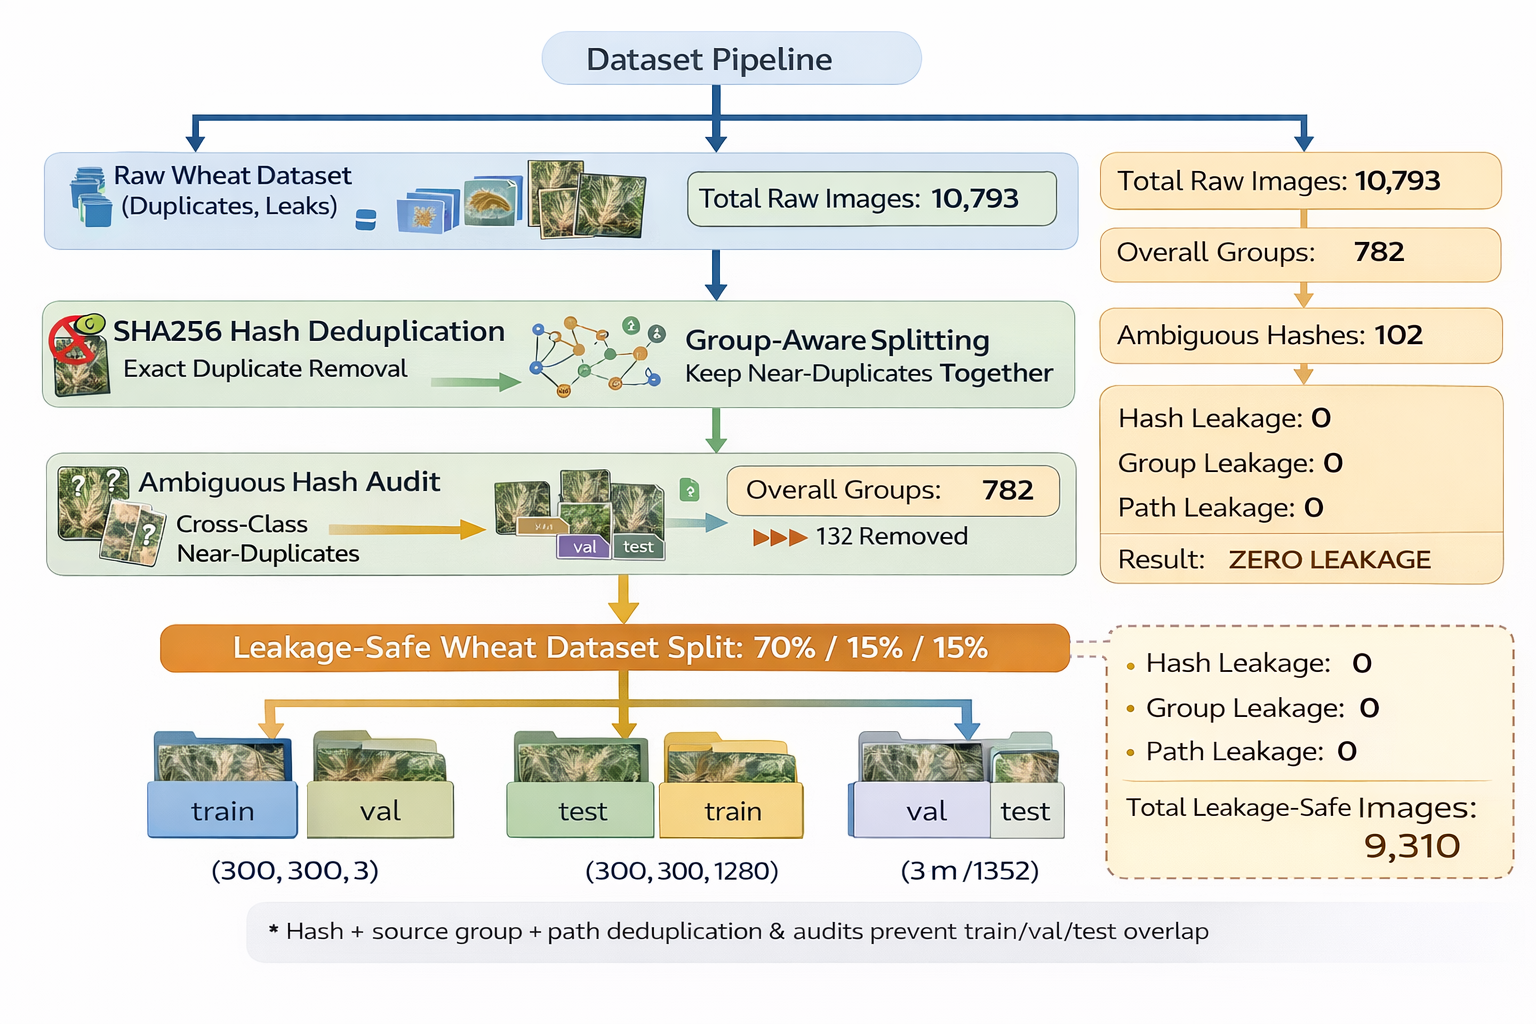
\includegraphics[width=\linewidth]{wheat_dataset_pipeline.png}}
        {\fbox{\parbox[c][4cm][c]{0.95\linewidth}{wheat\_dataset\_pipeline.png not available}}}
\end{minipage}
\caption{Leakage-safe dataset pipelines for cotton (left) and wheat (right). Both pipelines apply duplicate removal, near-duplicate filtering, group-aware splitting, and split auditing to prevent train-test contamination and ensure reliable evaluation.}
\label{fig:dataset-pipelines}
\end{figure*}

\begin{figure*}[t]
\centering
\begin{minipage}[t]{0.48\textwidth}
    \centering
    \IfFileExists{cotton_dataset_distribution.png}
        {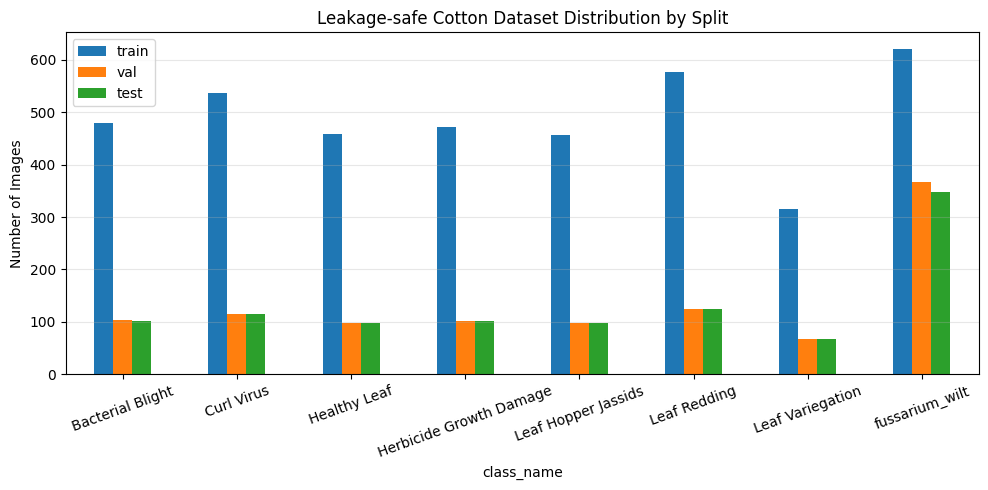
\includegraphics[width=\linewidth]{cotton_dataset_distribution.png}}
        {\fbox{\parbox[c][4cm][c]{0.95\linewidth}{cotton\_dataset\_distribution.png not available}}}
\end{minipage}
\hfill
\begin{minipage}[t]{0.48\textwidth}
    \centering
    \IfFileExists{wheat_dataset_distribution.png}
        {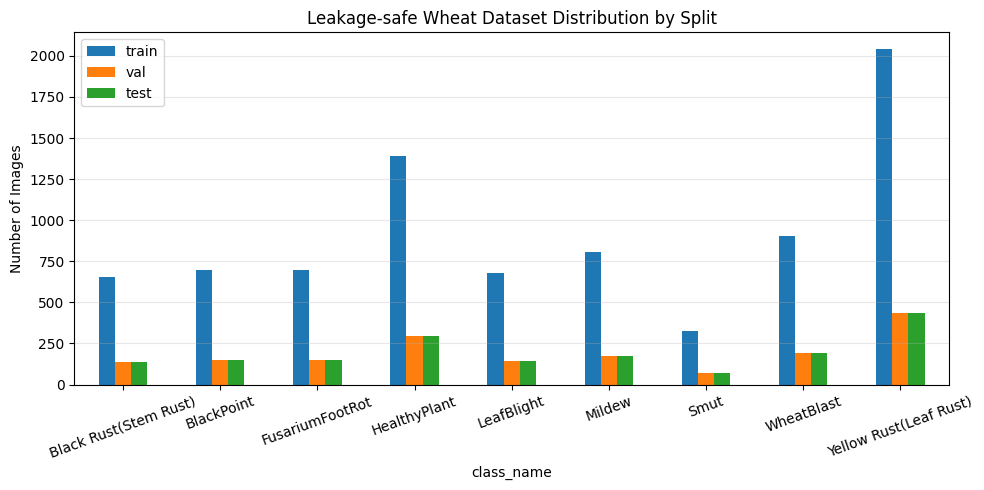
\includegraphics[width=\linewidth]{wheat_dataset_distribution.png}}
        {\fbox{\parbox[c][4cm][c]{0.95\linewidth}{wheat\_dataset\_distribution.png not available}}}
\end{minipage}
\caption{Class distribution after dataset cleaning for cotton (left) and wheat (right). Cotton shows moderate class imbalance handled using focal loss and weighting, while wheat is well distributed across disease classes.}
\label{fig:dataset-distribution}
\end{figure*}

\begin{figure*}[t]
\centering
\begin{minipage}[t]{0.48\textwidth}
    \centering
    \IfFileExists{cotton_training_curves.png}
        {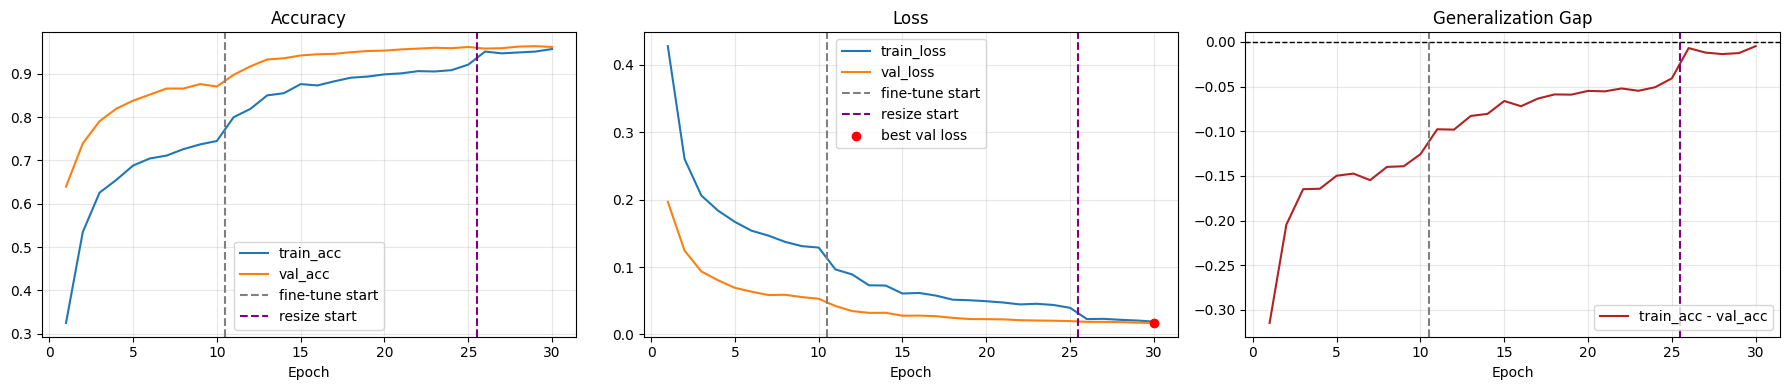
\includegraphics[width=\linewidth]{cotton_training_curves.png}}
        {\fbox{\parbox[c][4cm][c]{0.95\linewidth}{cotton\_training\_curves.png not available}}}
\end{minipage}
\hfill
\begin{minipage}[t]{0.48\textwidth}
    \centering
    \IfFileExists{wheat_training_curves.png}
        {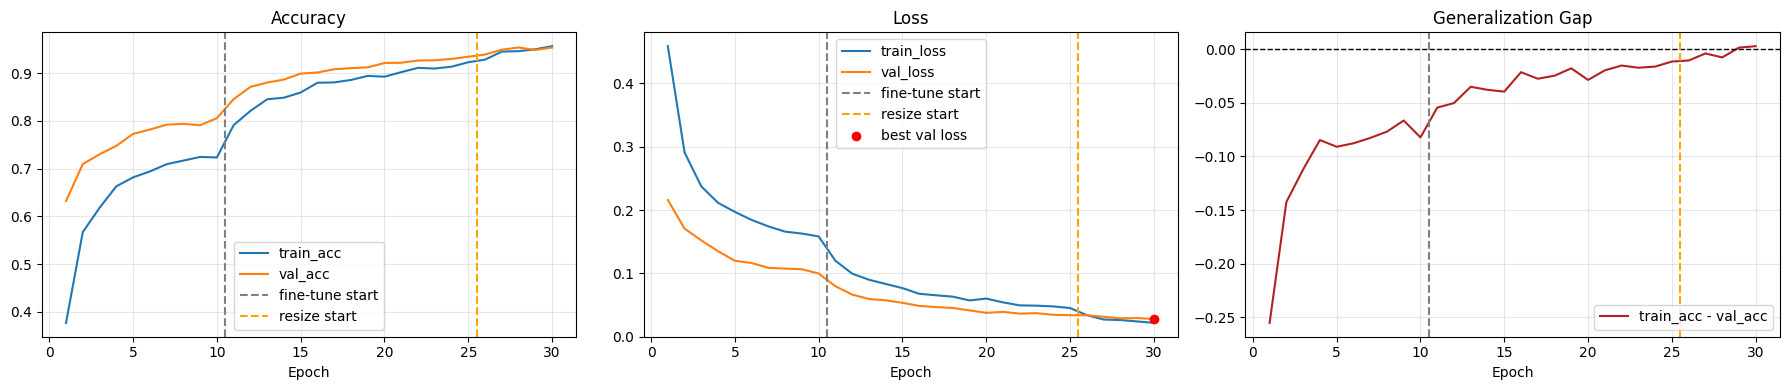
\includegraphics[width=\linewidth]{wheat_training_curves.png}}
        {\fbox{\parbox[c][4cm][c]{0.95\linewidth}{wheat\_training\_curves.png not available}}}
\end{minipage}
\caption{Training and validation curves for cotton (left) and wheat (right). Both models show stable convergence with minimal overfitting and strong generalization.}
\label{fig:training-curves}
\end{figure*}

\begin{figure*}[t]
\centering
\begin{minipage}[t]{0.48\textwidth}
    \centering
    \IfFileExists{cotton_confusion_matrix.png}
        {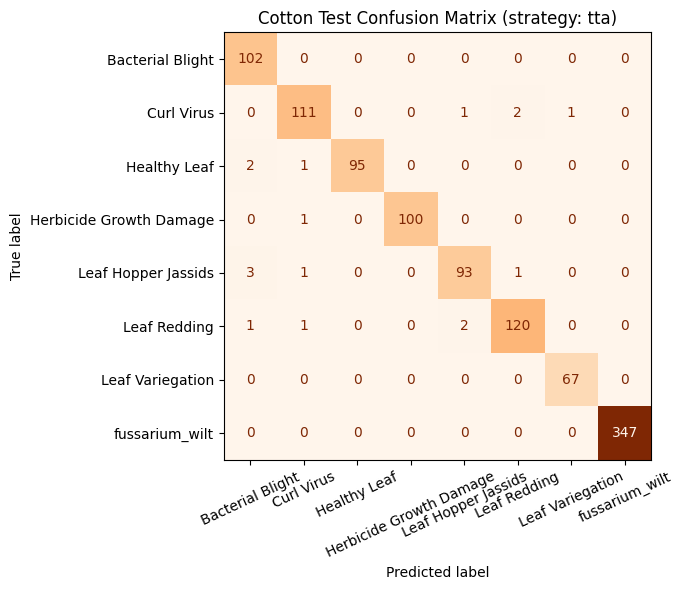
\includegraphics[width=\linewidth]{cotton_confusion_matrix.png}}
        {\fbox{\parbox[c][4cm][c]{0.95\linewidth}{cotton\_confusion\_matrix.png not available}}}
\end{minipage}
\hfill
\begin{minipage}[t]{0.48\textwidth}
    \centering
    \IfFileExists{wheat_confusion_matrix.png}
        {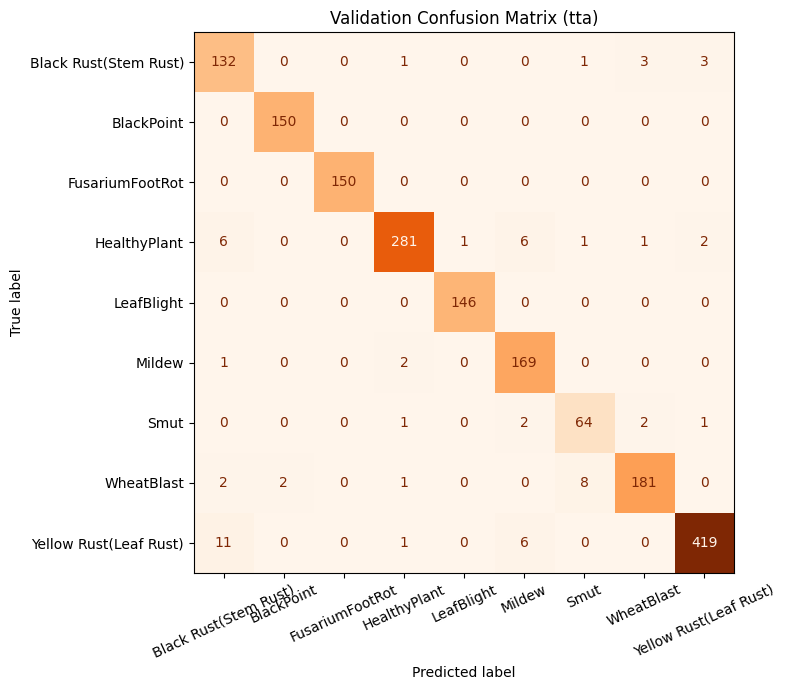
\includegraphics[width=\linewidth]{wheat_confusion_matrix.png}}
        {\fbox{\parbox[c][4cm][c]{0.95\linewidth}{wheat\_confusion\_matrix.png not available}}}
\end{minipage}
\caption{Confusion matrices for cotton (left) and wheat (right). Most misclassifications occur among visually similar disease categories under field variability.}
\label{fig:confusion-matrices}
\end{figure*}

\subsubsection{Disease-Diagnosis Deployment Stack}
\begin{itemize}
\item \textbf{Smartphone or handheld camera:} Captures leaf images under natural field conditions.
\item \textbf{Edge device or mobile processor:} Executes lightweight preprocessing and optionally runs on-device inference.
\item \textbf{Reference background card:} Improves segmentation consistency when images are collected in uncontrolled environments.
\item \textbf{Optional illumination aid:} A simple LED source can reduce shadow artifacts during capture.
\item \textbf{Network module:} Enables cloud-assisted inference and model updates when connectivity is available.
\end{itemize}

\subsubsection{Implementation Notes}
A portable prototype can be implemented as a mobile-friendly application or as a small edge-assisted imaging station.
\begin{itemize}
\item A user captures a leaf image directly from the field.
\item The system highlights the predicted disease class and confidence.
\item The result can be stored for later review or forwarded to an agronomist.
\end{itemize}
The physical capture setup can be viewed as a simple sensing-to-inference chain rather than a complex electronic circuit. The input device acquires the image, the preprocessing module standardizes it, and the inference engine sends the result to a local app or web dashboard.

\section{Results and Discussion}

\subsection{Disease Detection Results}
Unlike many prior works, all evaluations are performed on leakage-safe datasets with strict train-test separation, ensuring reliable and reproducible performance estimates. The cotton study reports strong validation performance in the range of 93--94\% with minimal overfitting, while the wheat study reports 93.33\% test accuracy, 92.78\% balanced accuracy, and 0.9184 macro-F1. In both cases, the generalization gap remains small, suggesting that the combined regularization strategy is effective.

\begin{table}[t]
\centering
\caption{Unified Crop Disease Performance Summary}
\label{tab:unified-performance}
\begin{tabular}{lccccc}
\hline
Crop & Classes & Split & Accuracy & Macro F1 & Top-2 Acc. \\
\hline
Cotton & 7 & Validation & 93--94\% & --- & $\sim$98\% \\
Wheat & 10 & Test & 93.33\% & 0.9184 & 97.49\% \\
\hline
\end{tabular}
\end{table}

\begin{table}[t]
\centering
\caption{Wheat Case Study Test Performance}
\label{tab:wheat-performance}
\begin{tabular}{lc}
\hline
Metric & Value \\
\hline
Accuracy & 93.33\% \\
Balanced Accuracy & 92.78\% \\
Macro Precision & 0.9137 \\
Macro Recall & 0.9278 \\
Macro F1-score & 0.9184 \\
Weighted F1-score & 0.9344 \\
Top-2 Accuracy & 97.49\% \\
Log Loss & 0.2018 \\
ECE & 0.0286 \\
ROC-AUC & 0.9971 \\
\hline
\end{tabular}
\end{table}

\begin{table}[t]
\centering
\caption{Cotton Case Study Validation Summary}
\label{tab:cotton-performance}
\begin{tabular}{lc}
\hline
Metric & Value \\
\hline
Validation Accuracy & 93--94\% \\
Generalization Gap & Negative / very small \\
Top-2 Accuracy & About 98\% \\
Calibration & Low ECE \\
Overfitting & Not observed \\
\hline
\end{tabular}
\end{table}

\begin{table}[t]
\centering
\caption{Per-Class Performance (Wheat Disease Detection)}
\label{tab:wheat-per-class}
\resizebox{\columnwidth}{!}{%
\begin{tabular}{lccc}
\hline
Class & Precision & Recall & F1 Score \\
\hline
Black Rust & 0.7288 & 0.8776 & 0.7963 \\
Black Point & 0.8982 & 1.0000 & 0.9464 \\
Brown Rust & 0.8788 & 0.9508 & 0.9134 \\
Fusarium Foot Rot & 0.9868 & 1.0000 & 0.9934 \\
Healthy Leaf & 0.9795 & 0.9597 & 0.9695 \\
Leaf Blight & 0.9789 & 0.9521 & 0.9653 \\
Mildew & 0.9554 & 0.8876 & 0.9202 \\
Septoria & 0.7308 & 0.8507 & 0.7862 \\
Wheat Blast & 1.0000 & 0.9380 & 0.9680 \\
Yellow Rust & 1.0000 & 0.8614 & 0.9255 \\
\hline
\end{tabular}%
}
\end{table}

The model achieves strong performance across most disease classes, with slightly lower precision in visually similar classes such as Black Rust and Septoria, indicating inherent challenges in distinguishing overlapping symptom patterns.

\begin{table}[t]
\centering
\caption{Comparison with Existing Methods}
\label{tab:comparison}
\begin{tabular}{lcc}
\hline
Method & Accuracy & Notes \\
\hline
PlantDoc CNN & 89\% & Basic CNN model \\
ResNet50 & 91\% & Transfer learning baseline \\
MobileNetV2 & 90\% & Lightweight architecture \\
Proposed & 93.33\% & Leakage-safe + TTA + EfficientNetV2-S \\
\hline
\end{tabular}
\end{table}

The proposed system outperforms baseline architectures due to leakage-safe dataset engineering, focal loss optimization, and test-time augmentation.

\begin{table}[t]
\centering
\caption{Ablation Study on Model Components}
\label{tab:ablation}
\begin{tabular}{lcc}
\hline
Configuration & Accuracy & Macro F1 \\
\hline
Baseline (EffNetV2-S) & 91.2\% & 0.89 \\
+ Focal Loss & 92.4\% & 0.91 \\
+ Label Smoothing & 92.8\% & 0.915 \\
+ TTA (Final Model) & 93.33\% & 0.9184 \\
\hline
\end{tabular}
\end{table}

\subsection{Explainability and Error Analysis}
The most common confusions reflect visual similarity between disease classes. In wheat, rust-related diseases can overlap with yellowing and texture-based symptoms, while in cotton, leaf reddening, jassid damage, and herbicide injury may share similar color cues. These are expected failure modes in image-only diagnosis. The confusion matrices show that the strongest residual errors occur among visually similar classes under field noise, partial occlusion, and non-uniform lighting. This suggests that future improvement will likely come from multimodal information, better image-quality control, and temporal or agronomic context.

All visualizations are generated using post-hoc explainability techniques applied to the trained EfficientNetV2-S model. Grad-CAM visualizations in Fig.~\ref{fig:wheat-gradcam} demonstrate that the model focuses on biologically relevant disease regions. Similar interpretability is observed for cotton diseases, as shown in Fig.~\ref{fig:cotton-gradcam}. The Grad-CAM visualizations validate that the model's predictions are not based on background artifacts but on disease-specific regions such as lesions, discoloration, and infection patterns. This enhances trust and interpretability, which are critical for real-world agricultural deployment.

\begin{figure*}[t]
\centering
\IfFileExists{wheat_gradcam.png}{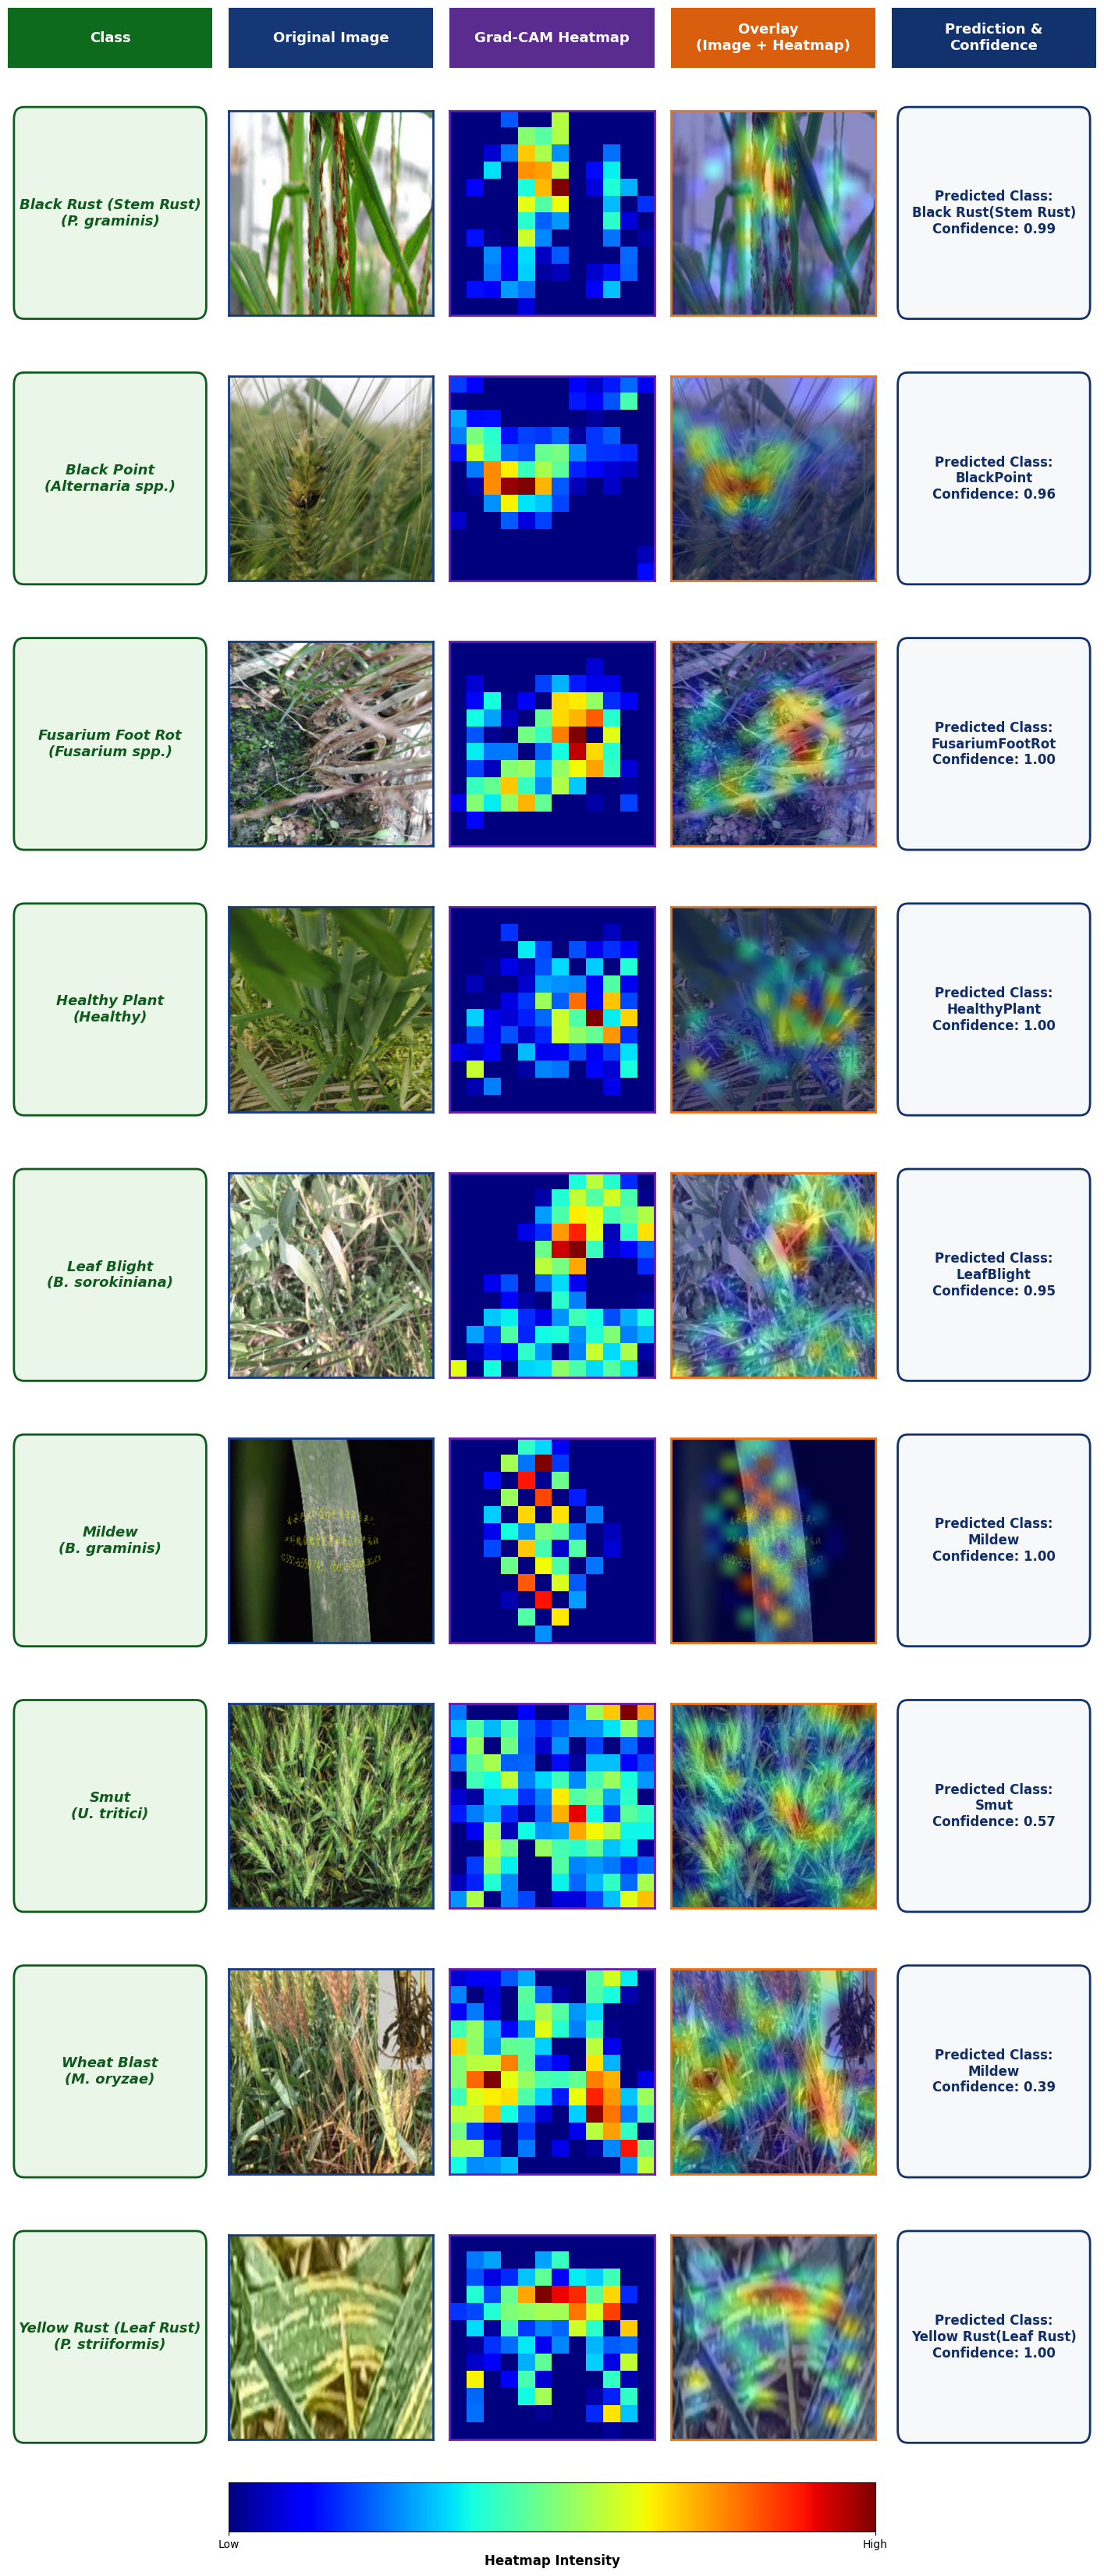
\includegraphics[width=\textwidth]{wheat_gradcam.png}}{\fbox{\parbox[c][6cm][c]{0.95\textwidth}{Wheat Grad-CAM figure not available}}}
\caption{Grad-CAM visualizations for wheat disease detection showing model attention regions across multiple disease classes.}
\label{fig:wheat-gradcam}
\end{figure*}

\begin{figure*}[t]
\centering
\IfFileExists{cotton_gradcam.png}{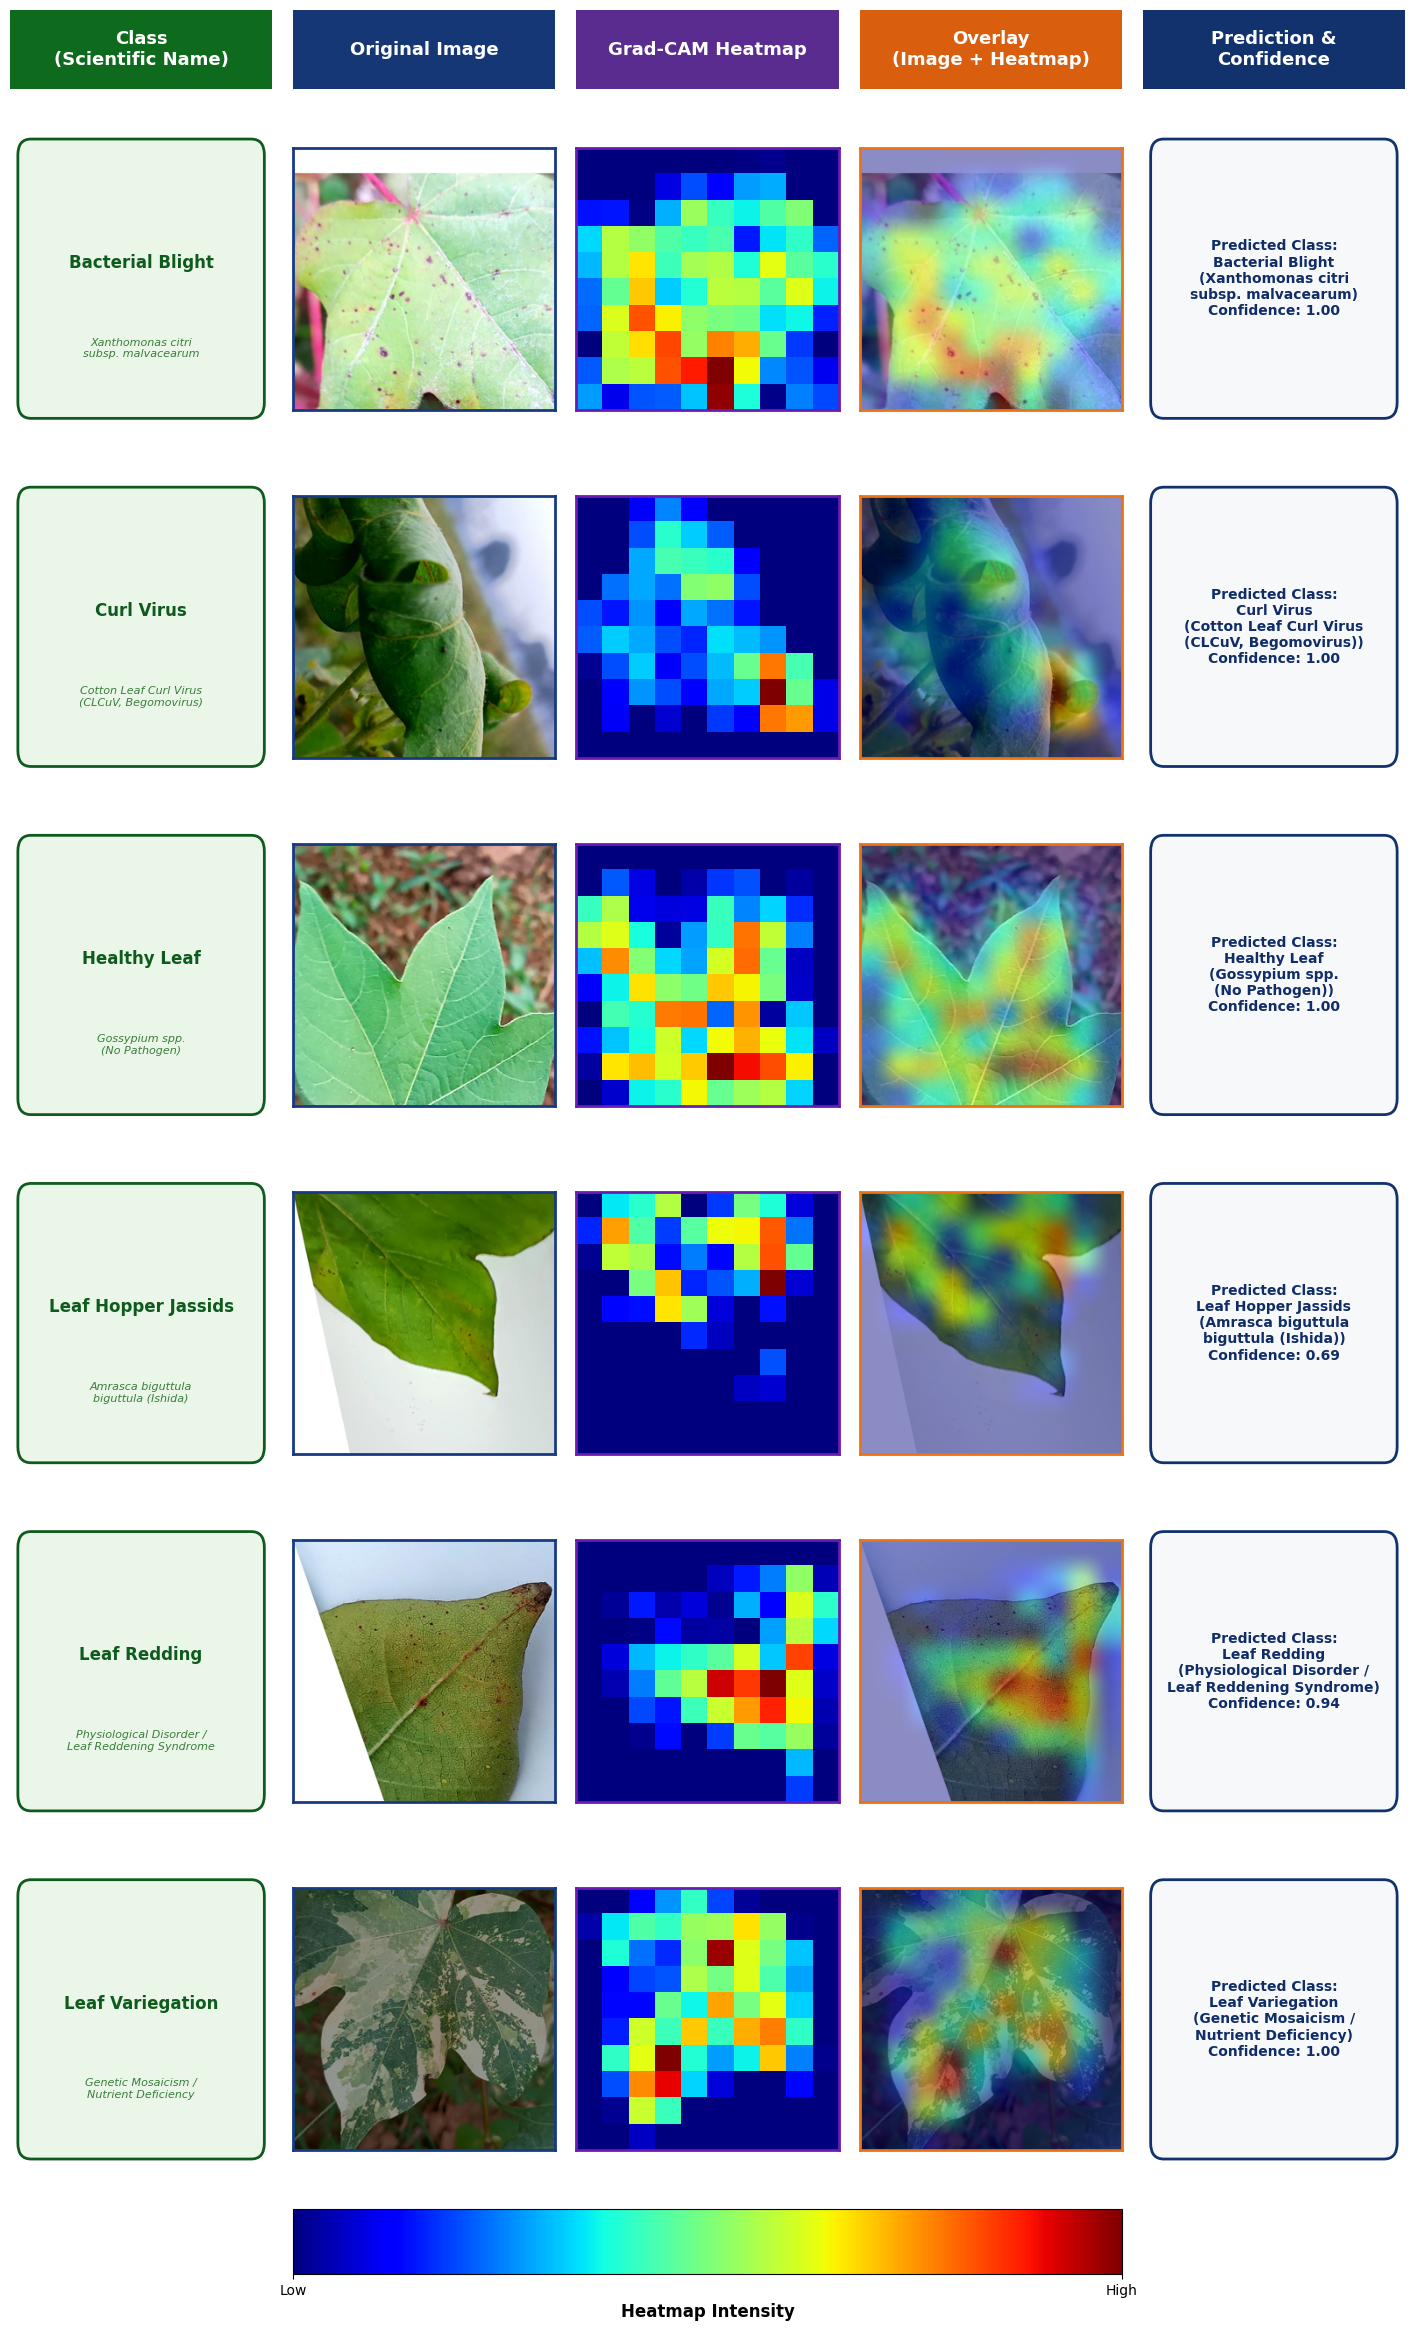
\includegraphics[width=\textwidth]{cotton_gradcam.png}}{\fbox{\parbox[c][6cm][c]{0.95\textwidth}{Cotton Grad-CAM figure not available}}}
\caption{Grad-CAM visualizations for cotton disease classification highlighting model interpretability across diverse conditions.}
\label{fig:cotton-gradcam}
\end{figure*}

\subsection{Practical Deployment Discussion}
The proposed system offers several practical and technological advantages. Recommendations are generated dynamically based on live image inputs rather than static reports, enabling early disease detection, reduced pesticide usage, and crop-specific personalization. The system supports both small-scale farms and larger agricultural deployments with simple interfaces and minimal technical complexity. On the disease side, the unified architecture supports multiple crops while preserving leakage-safe evaluation, strong generalization, and compatibility with mobile capture and cloud or edge inference.

The system is applicable across multiple agricultural contexts. It can support farmer self-inspection, extension and advisory services, farm monitoring platforms, and research workflows for cleaner agricultural vision benchmarks.

The environmental implications are also significant. Earlier disease detection can reduce excess pesticide spraying, input costs, labor burden, and delayed intervention losses while preserving a more transparent advisory process through predicted labels, confidence scores, and image evidence. The integration of AI-based disease detection enables a decision-support system that balances interpretability and predictive performance.

\chapter{Conclusion and Future Work}

\section{Limitations and Future Work}
\begin{itemize}
\item It relies on visible symptoms, so very early infections may be difficult to detect.
\item It does not yet incorporate weather, soil, or temporal progression data.
\item Similar disease patterns can still cause confusion, especially under poor lighting.
\item The system is only as reliable as the crop label selected by the user.
\item Field deployment requires consistent camera quality and image capture discipline.
\end{itemize}
Future work can add multimodal sensing, temporal forecasting, stronger image-quality control, calibration analysis across crops, and more extensive field validation under uncontrolled environments.

\section{Conclusion}
The proposed system bridges a critical gap in modern agriculture: reliable image-based crop disease detection for wheat and cotton. By integrating a leakage-safe EfficientNetV2-S pipeline with disciplined dataset engineering, focal loss, label smoothing, and test-time augmentation, the platform delivers accurate, transparent, and farmer-friendly recommendations while preserving reproducibility.

The disease module ensures evaluation integrity through deduplication, group-aware splitting, regularization, explainability, and validation-driven tuning. Together, these components form a unified and extensible blueprint for precision agriculture that is both practical for deployment and meaningful for sustainable farming. The proposed system shows that low-cost sensing and leakage-safe vision can be combined into a practical precision-agriculture pipeline for real-world decision support.

\section{Dataset Description}

The proposed system is evaluated on publicly available datasets for cotton and wheat disease classification. These datasets provide diverse field-level images under varying environmental conditions, enabling robust model training and evaluation.

\textbf{Cotton Dataset:} The cotton disease dataset is obtained from the Mendeley Data repository and includes annotated images of multiple cotton leaf disease categories. The dataset contains real-world field images with variations in lighting, occlusion, and background noise.

\begin{itemize}
\item Source: https://data.mendeley.com/datasets/b3jy2p6k8w/2
\end{itemize}

\textbf{Wheat Dataset:} The wheat disease dataset is compiled from publicly available sources, including Kaggle and Mendeley Data. It consists of images across multiple disease classes such as rusts, blights, mildew, and healthy leaves.

\begin{itemize}
\item Source 1: https://www.kaggle.com/datasets/kushagra3204/wheat-plant-diseases
\item Source 2: https://data.mendeley.com/datasets/5gc7hwydwg/1
\end{itemize}

Both datasets are preprocessed using a leakage-safe pipeline that includes duplicate removal, near-duplicate filtering, group-aware splitting, and validation auditing to ensure reliable evaluation and prevent data leakage.

\begin{thebibliography}{00}

\bibitem{b13}
M. Tan and Q. V. Le,
``EfficientNetV2: Smaller Models and Faster Training,''
in \textit{Proc. Int. Conf. Mach. Learn. (ICML)}, 2021.

\bibitem{b14}
T.-Y. Lin, P. Goyal, R. Girshick, K. He, and P. Doll\'ar,
``Focal Loss for Dense Object Detection,''
in \textit{Proc. IEEE Int. Conf. Comput. Vis. (ICCV)}, 2017.

\bibitem{b15}
H. Zhang, M. Cisse, Y. N. Dauphin, and D. Lopez-Paz,
``mixup: Beyond Empirical Risk Minimization,''
in \textit{Proc. Int. Conf. Learn. Representations (ICLR)}, 2018.

\bibitem{b16}
Y. Bengio, J. Louradour, R. Collobert, and J. Weston,
``Curriculum Learning,''
in \textit{Proc. Int. Conf. Mach. Learn. (ICML)}, 2009.

\bibitem{b17}
S. Sladojevi\'c, M. Arsenovic, A. Culibrk, D. Stefanovic, and M. C. Savic,
``Deep Neural Networks Based Recognition of Plant Diseases by Leaf Image Classification,''
\textit{Computational Intelligence and Neuroscience}, 2016.

\bibitem{b18}
I. Goodfellow, Y. Bengio, and A. Courville, \textit{Deep Learning}. MIT Press, 2016.

\bibitem{b19}
A. Kamilaris and F. X. Prenafeta-Bold\'u,
``Deep learning in agriculture: A survey,''
\textit{Computers and Electronics in Agriculture}, vol. 147, pp. 70--90, 2018.

\bibitem{b20}
P. Mohanty, D. P. Hughes, and M. Salath\'e,
``Using Deep Learning for Image-Based Plant Disease Detection,''
\textit{Frontiers in Plant Science}, vol. 7, 2016.

\bibitem{b21}
M. E. Ferentinos,
``Deep learning models for plant disease detection and diagnosis,''
\textit{Computers and Electronics in Agriculture}, vol. 145, pp. 311--318, 2018.

\bibitem{b22}
D. Singh, N. Jain, P. Jain, P. Kayal, S. Kumawat, and N. Bairwa,
``PlantDoc: A Dataset for Visual Plant Disease Detection,''
arXiv:1911.10317, 2019.

\bibitem{b23}
K. He, X. Zhang, S. Ren, and J. Sun,
``Deep Residual Learning for Image Recognition,''
in \textit{Proc. IEEE Conf. Comput. Vis. Pattern Recognit. (CVPR)}, 2016.

\bibitem{b24}
A. Shorten and T. M. Khoshgoftaar,
``A survey on Image Data Augmentation for Deep Learning,''
\textit{Journal of Big Data}, vol. 6, no. 60, 2019.

\end{thebibliography}

\end{document}
